\chapter{स्थलीय पौधों के जीवन-चक्र और जनन}\label{ch:b2:plant-life-cycles}

किसी दीवार पर \omterm{def:b2:plant-life-cycles:moss}{मॉस} का हरा गद्दा एक पौधा है; वसंत में उसमें से उठते भूरे
डंठल, हर एक बीजाणुओं के संपुट सहित, दूसरा पौधा हैं --- एक भिन्न व्यक्ति,
दुगुने गुणसूत्रों वाला, जो पहले में से उगता है और उसी पर जीता है। किसी
\omterm{def:b2:plant-life-cycles:fern}{फ़र्न} का पत्रक अपनी निचली सतह पर बीजाणु ढोता है, पर वे बीजाणु \omterm{def:b2:plant-life-cycles:fern}{फ़र्न} में
नहीं उगते: वे कुछ मिलिमीटर चौड़ी हृदयाकार हरी पपड़ी में उगते हैं, और
शुक्राणु तथा अंडाणु वहीं बनते हैं, और उसी पपड़ी से नया \omterm{def:b2:plant-life-cycles:fern}{फ़र्न} फूटता है।
हर स्थलीय पौधा इसी तरह दो कायाओं के बीच एकांतरित होता है, एक \omterm{def:b2:meiosis-heredity:meiosis}{अगुणित} और
एक \omterm{def:b2:meiosis-heredity:meiosis}{द्विगुणित}। यह अध्याय उस एकांतरण का शैवालों से बीज तक पीछा करता है,
और दिखाता है कि उसमें हुए परिवर्तनों की एक शृंखला ने --- \omterm{def:b2:meiosis-heredity:meiosis}{अगुणित} काया का
सिकुड़ना, \omterm{def:b2:plant-life-cycles:heterospory}{पराग} का आविष्कार, \omterm{def:b2:plant-life-cycles:heterospory}{बीजांड} का घेरा जाना, बीज --- जनन को जल से
कैसे मुक्त किया और पौधों को महाद्वीप ढकने दिए।

\section{जीवन-चक्र के तीन प्रकार}

\begin{definition}[अगुणितिक, द्विगुणितिक, अगुणित-द्विगुणितिक]\label{def:b2:plant-life-cycles:cycles}
\index{जीवन-चक्र}\index{पीढ़ी-एकांतरण}\index{युग्मकोद्भिद}\index{बीजाणुद्भिद}
हर लैंगिक जीवन-चक्र में एक \emph{निषेचन} होता है, जो गुणसूत्र-संख्या
दुगुनी करता है, और एक \emph{\omterm{def:b2:meiosis-heredity:meiosis}{अर्धसूत्री विभाजन}}, जो उसे आधी करता है;
और चक्र इसमें भिन्न हैं कि इन दोनों के बीच क्या होता है। किसी
\emph{अगुणितिक} चक्र में युग्मनज ही एकमात्र \omterm{def:b2:meiosis-heredity:meiosis}{द्विगुणित} कोशिका है और वह
तुरंत \omterm{def:b2:meiosis-heredity:meiosis}{अर्धसूत्री विभाजन} से गुज़रती है; जीव \omterm{def:b2:meiosis-heredity:meiosis}{अगुणित} है और उसके युग्मक
समसूत्री विभाजन से बनते हैं (\emph{Chlamydomonas}, अनेक शैवाल और कवक)।
किसी \emph{द्विगुणितिक} चक्र में \omterm{def:b2:meiosis-heredity:meiosis}{अर्धसूत्री विभाजन} सीधे युग्मक बनाता है,
युग्मक ही एकमात्र \omterm{def:b2:meiosis-heredity:meiosis}{अगुणित} कोशिकाएँ हैं, और जीव \omterm{def:b2:meiosis-heredity:meiosis}{द्विगुणित} है
(प्राणी, भूरी शैवाल \emph{Fucus})। किसी \emph{अगुणित-द्विगुणितिक}
चक्र में \omterm{def:b2:meiosis-heredity:meiosis}{अर्धसूत्री विभाजन} \emph{बीजाणु} बनाता है, जो समसूत्री विभाजन से
बढ़कर एक \omterm{def:b2:meiosis-heredity:meiosis}{अगुणित} जीव, \emph{युग्मकोद्भिद}, बनते हैं, जो समसूत्री विभाजन
से युग्मक बनाता है; और युग्मनज समसूत्री विभाजन से बढ़कर एक \omterm{def:b2:meiosis-heredity:meiosis}{द्विगुणित}
जीव, \emph{बीजाणुद्भिद}, बनता है, जो \omterm{def:b2:meiosis-heredity:meiosis}{अर्धसूत्री विभाजन} से बीजाणु बनाता
है। दो \omterm{def:b2:unicellular-diversity:unicellular}{बहुकोशिकीय} काएँ एकांतरित होती हैं --- यही
\emph{पीढ़ी-एकांतरण} है --- और यही हर स्थलीय पौधे का तथा अनेक शैवालों का
चक्र है।
\end{definition}

\begin{omfigure}
\begin{tikzpicture}[every node/.style={font=\scriptsize}, >=stealth]
  \foreach \dx/\title/\hap/\dip in {0/{अगुणितिक (\emph{Chlamydomonas})}/{अगुणित जीव ($n$)}/{युग्मनज ($2n$)}, 5.2/{द्विगुणितिक (प्राणी)}/{युग्मक ($n$)}/{द्विगुणित जीव ($2n$)}, 10.4/{अगुणित-द्विगुणितिक (पौधे)}/{युग्मकोद्भिद ($n$)}/{बीजाणुद्भिद ($2n$)}} {
    \begin{scope}[xshift=\dx cm]
      \node[anchor=south, font=\scriptsize\bfseries] at (2,2.5) {\title};
      \draw[thick, omDef, ->] (0.6,0.4) arc (200:340:1.5 and 1.0);
      \draw[thick, omThm, ->] (3.4,1.4) arc (20:160:1.5 and 1.0);
      \node[omDef, anchor=north] at (2,-0.3) {\hap};
      \node[omThm, anchor=south] at (2,2.05) {\dip};
      \node[anchor=south west] at (3.4,1.05) {निषेचन};
      \node[anchor=north east] at (0.55,0.75) {अर्धसूत्री विभाजन};
    \end{scope}
  }
  % emphasise the dominant phase by thickness of the arcs: draw thicker arcs
  \draw[line width=2.4pt, omDef, ->] (0.6,0.4) arc (200:340:1.5 and 1.0);
  \draw[line width=2.4pt, omThm, ->] (5.2+3.4,1.4) arc (20:160:1.5 and 1.0);
  \draw[line width=2.4pt, omDef, ->] (10.4+0.6,0.4) arc (200:340:1.5 and 1.0);
  \draw[line width=2.4pt, omThm, ->] (10.4+3.4,1.4) arc (20:160:1.5 and 1.0);
\end{tikzpicture}

{\small तीन \omterm{def:b2:plant-life-cycles:cycles}{जीवन-चक्र}। नीला: \omterm{def:b2:meiosis-heredity:meiosis}{अगुणित} प्रावस्था; लाल: \omterm{def:b2:meiosis-heredity:meiosis}{द्विगुणित}
प्रावस्था; और मोटे चाप \omterm{def:b2:unicellular-diversity:unicellular}{बहुकोशिकीय} काएँ हैं। हर चक्र
\omterm{def:b2:meiosis-heredity:meiosis}{अर्धसूत्री विभाजन} से एक बार और निषेचन से एक बार गुज़रता है; वे इसमें
भिन्न हैं कि कौन-सी प्रावस्था --- या दोनों --- किसी जीव में बढ़ती है।}
\end{omfigure}

\begin{proposition}[पीढ़ी-एकांतरण का अर्थ क्या है]\label{prop:b2:plant-life-cycles:alternation}
किसी स्थलीय पौधे में दोनों पीढ़ियाँ दो जीव हैं, एक ही जीव की दो अवस्थाएँ
नहीं: \omterm{def:b2:plant-life-cycles:cycles}{युग्मकोद्भिद} और \omterm{def:b2:plant-life-cycles:cycles}{बीजाणुद्भिद} के जीनोम भिन्न हैं
(\omterm{def:b2:meiosis-heredity:meiosis}{अगुणित} और \omterm{def:b2:meiosis-heredity:meiosis}{द्विगुणित}), काएँ भिन्न हैं, आकार प्रायः परिमाण की कई कोटियों
जितने भिन्न हैं, और हर एक किसी एक कोशिका से --- किसी बीजाणु या किसी
युग्मनज से --- समसूत्री विभाजन द्वारा विकसित होता है। \omterm{def:b2:plant-life-cycles:cycles}{युग्मकोद्भिद}
\omterm{def:b2:unicellular-diversity:unicellular}{बहुकोशिकीय} अंगों में युग्मक बनाता है, \emph{पुंधानियों} (शुक्राणु) और
\emph{स्त्रीधानियों} (हर एक में एक अंडाणु, ऐसी सुराही में जिसकी गर्दन से
होकर शुक्राणु नीचे तैरता है); और \omterm{def:b2:plant-life-cycles:cycles}{बीजाणुद्भिद} \emph{बीजाणुधानियों} में
बीजाणु बनाता है। स्थलीय पौधों में यह संतुलन खिसकता है: \omterm{def:b2:plant-life-cycles:moss}{मॉसों} में
\omterm{def:b2:plant-life-cycles:cycles}{युग्मकोद्भिद} ही पौधा है और \omterm{def:b2:plant-life-cycles:cycles}{बीजाणुद्भिद} एक आश्रित डंठल; \omterm{def:b2:plant-life-cycles:fern}{फ़र्नों} में
\omterm{def:b2:plant-life-cycles:cycles}{बीजाणुद्भिद} ही पौधा है और \omterm{def:b2:plant-life-cycles:cycles}{युग्मकोद्भिद} एक स्वतंत्र पपड़ी; और बीज-पौधों
में \omterm{def:b2:plant-life-cycles:cycles}{युग्मकोद्भिद} घटकर \omterm{def:b2:plant-life-cycles:cycles}{बीजाणुद्भिद} के ऊतकों में छिपी कुछ ही कोशिकाएँ रह
जाता है --- यानी \omterm{def:b2:plant-life-cycles:heterospory}{पराग} कण और \omterm{def:b2:plant-life-cycles:heterospory}{बीजांड} की अंतर्वस्तु।
\end{proposition}
\begin{proof}[प्रमाण-सामग्री]
हॉफ़माइस्टर (1851) ने \omterm{def:b2:plant-life-cycles:moss}{मॉसों}, \omterm{def:b2:plant-life-cycles:fern}{फ़र्नों}, हॉर्सटेलों और क्लबमॉसों के बीजाणु
अंकुरित किए, उनसे बनी छोटी हरी कायाओं का विकास देखा, उन पर पुंधानियाँ और
स्त्रीधानियाँ पाईं, और \omterm{def:b2:plant-life-cycles:moss}{स्त्रीधानी} के भीतर निषेचित अंडाणु से
भ्रूण को बीजाणुधारी पौधे में बढ़ते देखा। फिर उन्होंने दिखाया
कि किसी शंकुधारी के \omterm{def:b2:plant-life-cycles:heterospory}{बीजांड} में भी वही संरचनाएँ हैं, पर घटी हुई
--- ऐसे ऊतक के भीतर स्त्रीधानियाँ जो रोका गया \omterm{def:b2:plant-life-cycles:cycles}{युग्मकोद्भिद} है --- और
यों कि \omterm{def:b2:plant-life-cycles:moss}{मॉस}, \omterm{def:b2:plant-life-cycles:fern}{फ़र्न} और बीज-पौधे एक ही चक्र वाली एक ही शृंखला हैं।
वे गुणसूत्र-गणनाएँ जिन्होंने दोनों पीढ़ियों को समझाया (स्ट्रासबुर्गर,
1894) चालीस वर्ष बाद आईं।
\end{proof}

\section{मॉस: युग्मकोद्भिद ही पौधा है}

\begin{definition}[मॉस का जीवन-चक्र]\label{def:b2:plant-life-cycles:moss}
\index{मॉस}\index{प्रोटोनीमा}\index{स्त्रीधानी}\index{पुंधानी}
मॉस का कोई \emph{बीजाणु} अंकुरित होकर एक शाखित हरा तंतु बनता है,
\emph{प्रोटोनीमा}, जिससे मुकुल उगकर पत्तीदार प्ररोह बनते हैं --- यानी
\emph{\omterm{def:b2:plant-life-cycles:cycles}{युग्मकोद्भिद}}, जो कुछ सेंटीमीटर ऊँचा होता है, जिसमें न सच्ची जड़ें
हैं, न जाइलम, न फ्लोएम, जो मूलाभासों से टिका रहता है और अपनी पूरी सतह से
जल खींचता है। अपने प्ररोह-शीर्षों पर वह \emph{पुंधानियाँ} ढोता है, जो
द्विकशाभी शुक्राणु वर्षा या ओस की झिल्ली में छोड़ती हैं, और
\emph{स्त्रीधानियाँ}, जिनमें से हर एक की गर्दन के तल पर एक अंडाणु है; वे
शुक्राणु अधिक से अधिक कुछ सेंटीमीटर तैरते हैं, रासायनिक आकर्षियों की
राह पर, और वहीं अंडाणु को निषेचित कर देते हैं। युग्मनज बढ़कर
\emph{\omterm{def:b2:plant-life-cycles:cycles}{बीजाणुद्भिद}} बनता है: \omterm{def:b2:plant-life-cycles:cycles}{युग्मकोद्भिद} में धँसा एक पाद, एक डंठल
(\emph{सीटा}), और एक \emph{संपुट} जिसमें \omterm{def:b2:meiosis-heredity:meiosis}{अर्धसूत्री विभाजन} दसियों हज़ार
बीजाणु बनाता है, जो शुष्क हवा में खुलने वाले जलग्राही दाँतों के छल्ले से
झड़ते हैं। \omterm{def:b2:plant-life-cycles:cycles}{बीजाणुद्भिद} थोड़ा प्रकाशसंश्लेषण करता है पर पलता
\omterm{def:b2:plant-life-cycles:cycles}{युग्मकोद्भिद} से अपने पाद के रास्ते ही है और कभी अकेला नहीं जीता।
\end{definition}

\begin{omfigure}
\begin{tikzpicture}[every node/.style={font=\scriptsize}, >=stealth]
  \node[draw, rounded corners, fill=omDef!12, align=center] (spore) at (0,3) {बीजाणु ($n$)};
  \node[draw, rounded corners, fill=omDef!12, align=center] (proto) at (3.2,3) {प्रोटोनीमा};
  \node[draw, rounded corners, fill=omDef!12, align=center] (gam) at (6.6,3) {पत्तीदार युग्मकोद्भिद ($n$)\\पुंधानियाँ और स्त्रीधानियाँ};
  \node[draw, rounded corners, fill=omDef!12, align=center] (gametes) at (11.2,3) {शुक्राणु और अंडाणु ($n$)};
  \node[draw, rounded corners, fill=omThm!12, align=center] (zyg) at (11.2,0.8) {युग्मनज ($2n$)};
  \node[draw, rounded corners, fill=omThm!12, align=center] (sporo) at (6.6,0.8) {बीजाणुद्भिद ($2n$)\\पाद, सीटा, संपुट};
  \node[draw, rounded corners, fill=omThm!12, align=center] (cap) at (2.4,0.8) {संपुट में अर्धसूत्री विभाजन};
  \draw[->, thick] (spore) -- (proto) node[midway, above] {समसूत्री विभाजन};
  \draw[->, thick] (proto) -- (gam);
  \draw[->, thick] (gam) -- (gametes) node[midway, above] {समसूत्री विभाजन};
  \draw[->, thick] (gametes) -- (zyg) node[pos=0.3, right, align=left] {जल की झिल्ली में\\निषेचन};
  \draw[->, thick] (zyg) -- (sporo) node[midway, above] {समसूत्री विभाजन};
  \draw[->, thick] (sporo) -- (cap);
  \draw[->, thick] (cap) -| (spore) ;
  \node[omDef, anchor=west] at (-1.9,3.9) {अगुणित};
  \node[omThm, anchor=west] at (-1.9,-0.1) {द्विगुणित};
  \draw[gray, dashed] (-1.9,1.9) -- (13.2,1.9);
\end{tikzpicture}

{\small \omterm{def:b2:plant-life-cycles:moss}{मॉस} का चक्र। पत्तीदार पौधा \omterm{def:b2:meiosis-heredity:meiosis}{अगुणित} \omterm{def:b2:plant-life-cycles:cycles}{युग्मकोद्भिद} है;
\omterm{def:b2:plant-life-cycles:cycles}{बीजाणुद्भिद} उस पर उगता डंठल और संपुट है, जो उसी से पलता है
और \omterm{def:b2:meiosis-heredity:meiosis}{अर्धसूत्री विभाजन} से बीजाणु बनाता है।}
\end{omfigure}

\begin{omfigure}
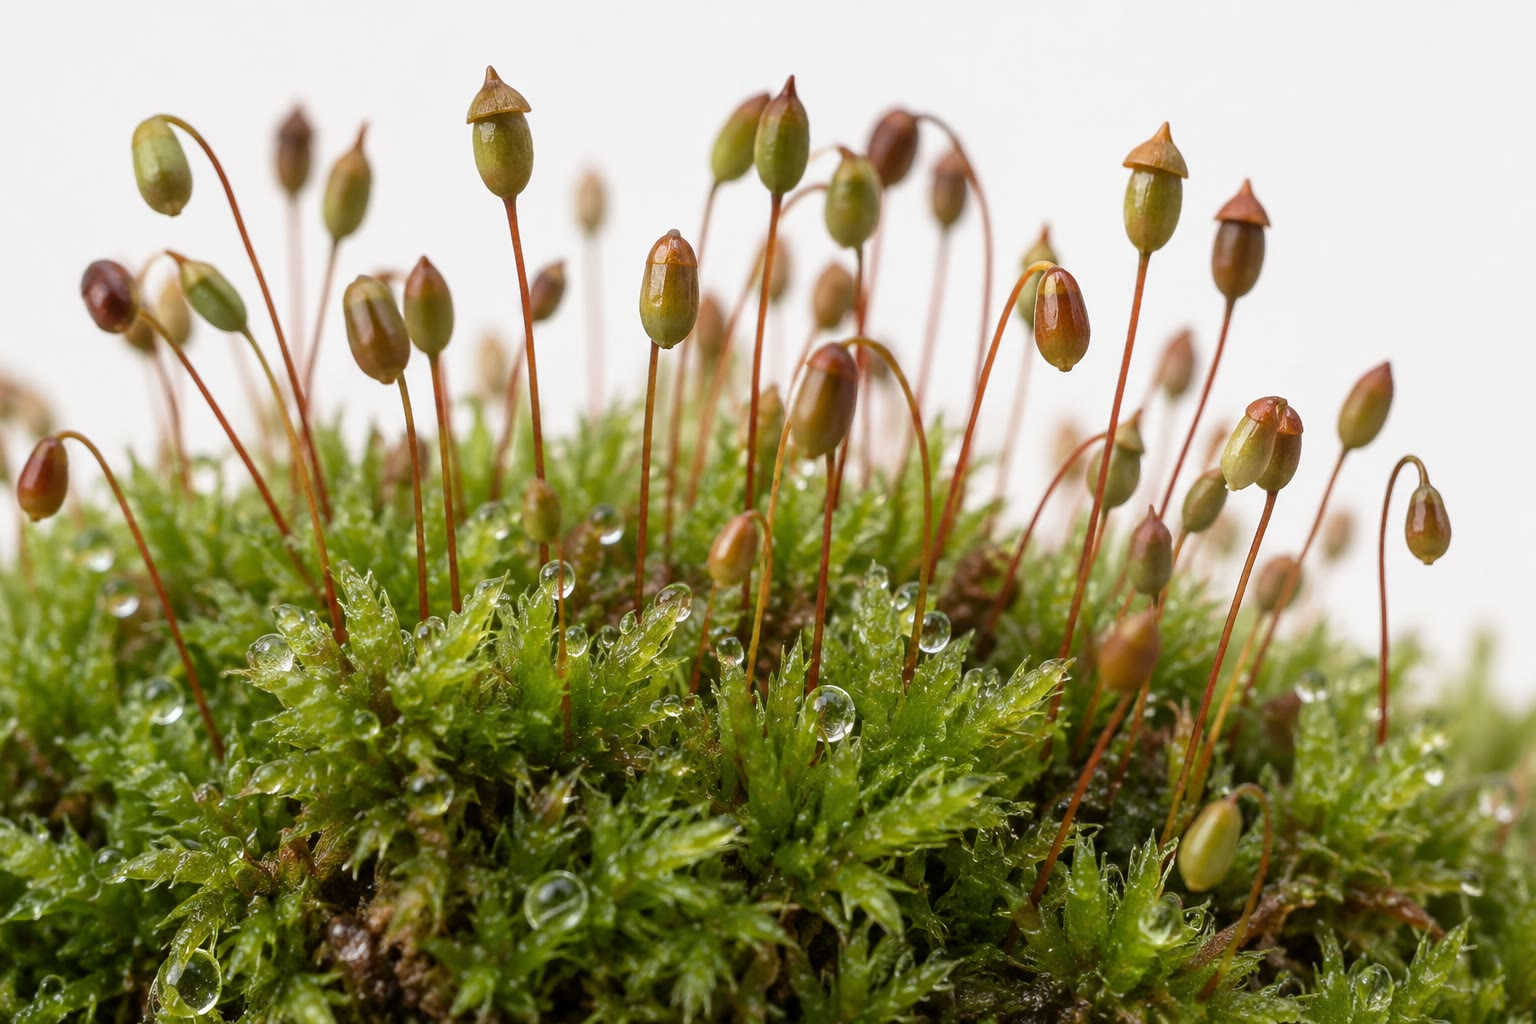
\includegraphics[width=0.6\linewidth]{images/book4/ai/b4-05-moss-sporophytes.jpg}

{\small वसंत में \omterm{def:b2:plant-life-cycles:moss}{मॉस} का एक गद्दा: हरे प्ररोह
\omterm{def:b2:plant-life-cycles:cycles}{युग्मकोद्भिद} हैं, और संपुट सहित हर लालिमा लिए डंठल किसी निषेचित अंडाणु
से उगा \omterm{def:b2:plant-life-cycles:cycles}{बीजाणुद्भिद} है, जो अब भी उसी प्ररोह से जुड़ा है
जिसने वह अंडाणु बनाया था।}
\end{omfigure}

\begin{example}[तैरते शुक्राणुओं की क़ीमत]\label{ex:b2:plant-life-cycles:sperm}
\omterm{def:b2:plant-life-cycles:moss}{मॉस} का शुक्राणु लगभग \qty{100}{\micro m/s} से तैरता है; \qty{2}{cm}
दूर की किसी \omterm{def:b2:plant-life-cycles:moss}{स्त्रीधानी} तक पहुँचने के लिए उसे \qty{200}{s} तक अटूट
जल-झिल्ली चाहिए --- वर्षा की एक बौछार, भारी ओस। इसलिए निषेचन
गीले मौसम तक और छोटी दूरियों तक सीमित है, और अधिकांश
\omterm{def:b2:plant-life-cycles:moss}{मॉस}, \omterm{def:b2:plant-life-cycles:fern}{फ़र्न} तथा उनके सगे नम स्थानों में रहते हैं या गीले मौसम में जनन
करते हैं; कुछ \omterm{def:b2:plant-life-cycles:moss}{मॉसों} की पुंधानियाँ ऐसे छींटा-प्याले में बैठती हैं जिसका
आकार वर्षा की बूँदें, और उनमें ढोए शुक्राणु, आधा मीटर तक उछाल देता है।
यही निर्भरता है जिससे बीज-पौधे बच निकले।
\end{example}

\section{फ़र्न: बीजाणुद्भिद ही पौधा है}

\begin{definition}[फ़र्न का जीवन-चक्र]\label{def:b2:plant-life-cycles:fern}
\index{फ़र्न}\index{प्रोथैलस}\index{सोरस}\index{बीजाणुधानी}
फ़र्न ही \emph{\omterm{def:b2:plant-life-cycles:cycles}{बीजाणुद्भिद}} है: जड़ों, जाइलम और फ्लोएम
वाला एक प्रकंद, और पत्रक। उर्वर पत्रकों की निचली सतह पर
\emph{बीजाणुधानियों} के गुच्छ (\emph{सोरस}, प्रायः किसी रक्षक झिल्ली के
नीचे) हर एक \omterm{def:b2:meiosis-heredity:meiosis}{अर्धसूत्री विभाजन} से 64 बीजाणु बनाते हैं और उन्हें
मोटी-भित्ति कोशिकाओं के सूखते छल्ले की चटक से उछाल देते हैं। जो बीजाणु
नम मिट्टी पर गिरे वह \emph{प्रोथैलस} में उगता है: कुछ मिलिमीटर चौड़ा
हृदयाकार हरा \omterm{def:b2:plant-life-cycles:cycles}{युग्मकोद्भिद}, एक कोशिका मोटा, मूलाभासों सहित, जो कुछ
सप्ताह स्वतंत्र जीता है। वह अपनी निचली सतह पर पुंधानियाँ और
स्त्रीधानियाँ ढोता है; शुक्राणु मिट्टी की झिल्ली में तैरकर अंडाणु तक
जाते हैं; युग्मनज बढ़कर ऐसा नया \omterm{def:b2:plant-life-cycles:cycles}{बीजाणुद्भिद} बनता है जो अपना पहला भोजन
प्रोथैलस से लेता है और फिर जड़ पकड़ लेता है, और प्रोथैलस मर जाता है।
दोनों पीढ़ियाँ स्वतंत्र हैं, पर असमान: \omterm{def:b2:plant-life-cycles:cycles}{बीजाणुद्भिद} दशकों जीता है और
मीटरों ऊँचा हो सकता है, \omterm{def:b2:plant-life-cycles:cycles}{युग्मकोद्भिद} सप्ताहों और मिलिमीटरों का।
\end{definition}

\begin{omfigure}
\begin{tikzpicture}[every node/.style={font=\scriptsize}, >=stealth]
  \node[draw, rounded corners, fill=omThm!12, align=center] (fern) at (0,3) {फ़र्न का पौधा, बीजाणुद्भिद ($2n$)\\जड़ें, प्रकंद, पत्रक};
  \node[draw, rounded corners, fill=omThm!12, align=center] (sor) at (5.4,3) {सोरसों में बीजाणुधानियाँ\\(पत्रकों के नीचे)};
  \node[draw, rounded corners, fill=omDef!12, align=center] (spore) at (10.4,3) {बीजाणु ($n$)\\प्रति बीजाणुधानी 64};
  \node[draw, rounded corners, fill=omDef!12, align=center] (pro) at (10.4,0.6) {प्रोथैलस ($n$)\\स्वतंत्र, मिलिमीटर-आकार\\पुंधानियाँ, स्त्रीधानियाँ};
  \node[draw, rounded corners, fill=omDef!12, align=center] (gam) at (5.4,0.6) {शुक्राणु और अंडाणु ($n$)};
  \node[draw, rounded corners, fill=omThm!12, align=center] (zyg) at (0,0.6) {युग्मनज ($2n$), फिर\\प्रोथैलस पर\\नया बीजाणुद्भिद};
  \draw[->, thick] (fern) -- (sor);
  \draw[->, thick] (sor) -- (spore) node[midway, above] {अर्धसूत्री विभाजन};
  \draw[->, thick] (spore) -- (pro) node[midway, right] {समसूत्री विभाजन};
  \draw[->, thick] (pro) -- (gam) node[midway, above] {समसूत्री विभाजन};
  \draw[->, thick] (gam) -- (zyg) node[midway, above, align=center] {निषेचन\\(तैरते शुक्राणु)};
  \draw[->, thick] (zyg) -- (fern) node[midway, right] {समसूत्री विभाजन};
  \draw[gray, dashed] (7.9,-0.5) -- (7.9,4.0);
  \node[omThm, anchor=south] at (2.7,3.9) {द्विगुणित पीढ़ी};
  \node[omDef, anchor=south] at (10.4,3.9) {अगुणित पीढ़ी};
\end{tikzpicture}

{\small \omterm{def:b2:plant-life-cycles:fern}{फ़र्न} का चक्र। जिस पौधे को हम \omterm{def:b2:plant-life-cycles:fern}{फ़र्न} कहते हैं वह \omterm{def:b2:meiosis-heredity:meiosis}{द्विगुणित}
\omterm{def:b2:plant-life-cycles:cycles}{बीजाणुद्भिद} है; \omterm{def:b2:meiosis-heredity:meiosis}{अगुणित} \omterm{def:b2:plant-life-cycles:cycles}{युग्मकोद्भिद} एक अल्पजीवी \omterm{def:b2:plant-life-cycles:fern}{प्रोथैलस} है जिस
पर शुक्राणु तैरकर अंडाणुओं तक जाते हैं।}
\end{omfigure}

\begin{omfigure}
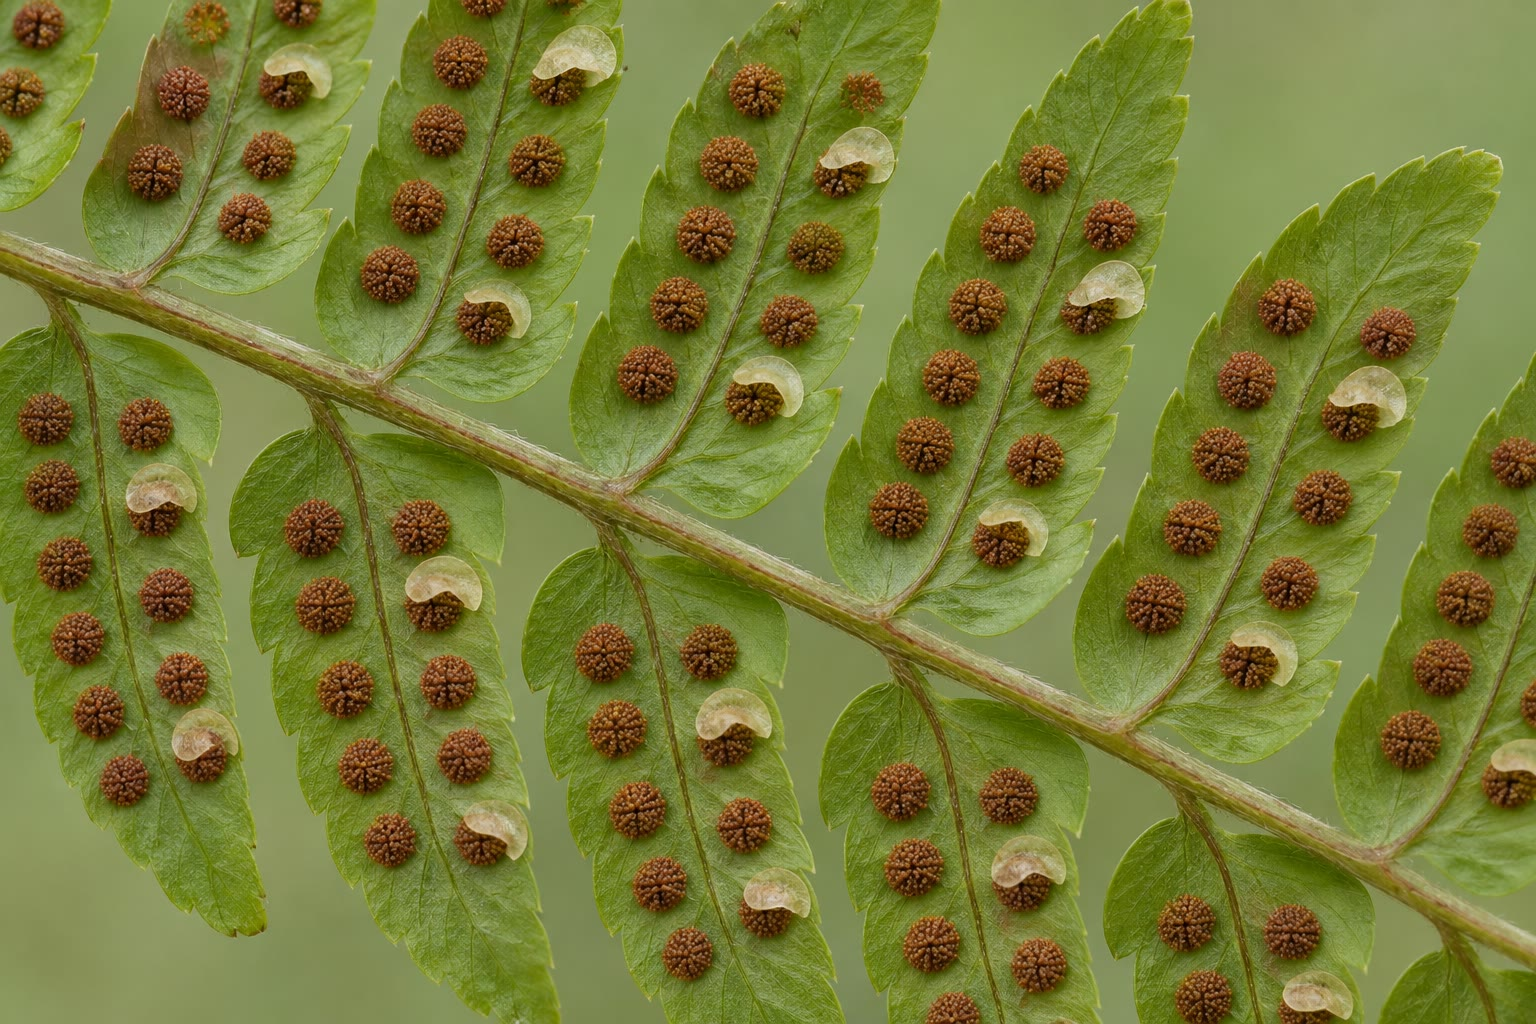
\includegraphics[width=0.6\linewidth]{images/book4/ai/b4-05-fern-sori.jpg}

{\small किसी उर्वर \omterm{def:b2:plant-life-cycles:fern}{फ़र्न} पत्रक की निचली सतह: हर भूरा बिंदु एक
\omterm{def:b2:plant-life-cycles:fern}{सोरस} है, यानी बीजाणुधानियों का गुच्छ, और कुछ अब भी उस झिल्ली से ढके हैं
जो उन्हें पकने तक बचाती है।}
\end{omfigure}

\begin{theorem}[किसी बीजाणु का प्रकीर्णन]\label{thm:b2:plant-life-cycles:dispersal}
\index{बीजाणु प्रकीर्णन}
$r$ त्रिज्या और $\rho_s$ घनत्व का कोई बीजाणु, जो $h$ ऊँचाई से $u$ चाल की
किसी क्षैतिज वायु में छोड़ा जाए, स्टोक्स सीमांत चाल
$v_s = 2r^2(\rho_s - \rho_{\text{वायु}})g/9\eta_{\text{वायु}}$ से गिरता
है और, स्थिर-स्तरित वायु में, इतनी दूरी पर उतरता है:
\[
x = \frac{u\,h}{v_s}
\]
यानी पौधे से इतनी दूर। \qty{15}{\micro m} त्रिज्या और
\qty{1100}{kg/m^3} घनत्व का कोई \omterm{def:b2:plant-life-cycles:fern}{फ़र्न} बीजाणु ($\eta_{\text{वायु}} = \qty{1.8e-5}{Pa.s}$)
\qty{3}{cm/s} से गिरता है; \qty{0.5}{m} पर के किसी पत्रक से
\qty{2}{m/s} की वायु में वह लगभग \qty{30}{m} जाता है, और किसी हवादार दिन
की विक्षुब्ध वायु में, जो बीजाणुओं के एक अंश को छोड़े जाने की ऊँचाई से
कहीं ऊपर उठा देती है, कुछ सैकड़ों किलोमीटर जाते हैं --- और इसीलिए
समुद्री द्वीपों की \omterm{def:b2:plant-life-cycles:fern}{फ़र्न} वनस्पति समृद्ध है और उनकी बीज-पौधा वनस्पति
दरिद्र।
\end{theorem}
\begin{proof}
गिरने का काल $h/v_s$ है (बीजाणु अपनी सीमांत चाल माइक्रोसेकंडों में पा
लेता है), और उस दौरान वायु उसे $u\,h/v_s$ ले जाती है। सीमांत
चाल स्टोक्स कर्षण $6\pi\eta r
v_s$ को भार घटा उत्प्लावन $\tfrac43\pi r^3(\rho_s -
\rho_{\text{वायु}})g$ से संतुलित करने पर निकलती है, जैसा \cref{ch:b2:unicellular-diversity} में।
\end{proof}

\section{बीज-पौधे: युग्मकोद्भिद छिपा हुआ है}

\begin{definition}[विषमबीजाणुता, पराग, बीजांड]\label{def:b2:plant-life-cycles:heterospory}
\index{विषमबीजाणुता}\index{पराग}\index{बीजांड}\index{लघुबीजाणु}\index{गुरुबीजाणु}
\omterm{def:b2:plant-life-cycles:moss}{मॉस} और अधिकांश \omterm{def:b2:plant-life-cycles:fern}{फ़र्न} \emph{समबीजाणुक} हैं: एक ही प्रकार का बीजाणु, एक ही
प्रकार का \omterm{def:b2:plant-life-cycles:cycles}{युग्मकोद्भिद} जो दोनों लिंग ढोता है। बीज-पौधे (और कुछ
\omterm{def:b2:plant-life-cycles:fern}{फ़र्न} तथा क्लबमॉस) \emph{विषमबीजाणुक} हैं: \emph{लघुबीजाणु},
छोटे और अनेक, नर \omterm{def:b2:plant-life-cycles:cycles}{युग्मकोद्भिदों} में उगते हैं; \emph{गुरुबीजाणु}, बड़े
और थोड़े, मादा \omterm{def:b2:plant-life-cycles:cycles}{युग्मकोद्भिदों} में। बीज-पौधों में दोनों घटकर
लगभग कुछ भी नहीं रह जाते और कोई भी \omterm{def:b2:plant-life-cycles:cycles}{बीजाणुद्भिद} के ऊतक अपने बल पर नहीं
छोड़ता। नर \omterm{def:b2:plant-life-cycles:cycles}{युग्मकोद्भिद} \emph{पराग कण} है: ऐसा लघुबीजाणु
जो अपनी भित्ति के भीतर दो या तीन बार विभाजित हो चुका है, और वायु या
प्राणियों से मादा अंग तक पहुँचाया जाता है, जहाँ वह एक \emph{पराग नलिका}
उगाता है और अपने शुक्राणु पहुँचा देता है --- कोई जल नहीं चाहिए। मादा
\omterm{def:b2:plant-life-cycles:cycles}{युग्मकोद्भिद} गुरुबीजाणुधानी के भीतर विकसित होता है, जो जनक पर ही रहती है
और एक छिद्र, \emph{बीजांडद्वार}, वाले एक या दो \emph{अध्यावरणों} में
घिरी रहती है: यह पूरी संरचना ही \emph{बीजांड} है। निषेचन के
बाद बीजांड \emph{बीज} बन जाता है: एक भ्रूण
\omterm{def:b2:plant-life-cycles:cycles}{बीजाणुद्भिद}, भोजन का एक भंडार, और अध्यावरणों से बना एक आवरण,
जो परिस्थितियाँ ठीक होने तक प्रसुप्त रहता है।
\end{definition}

\begin{omfigure}
\begin{tikzpicture}[every node/.style={font=\scriptsize}]
  % ovule in section
  \draw[thick, fill=omExo!25] (0,0) ellipse (1.6 and 2.2);
  \draw[thick, fill=omExo!10] (0,0) ellipse (1.25 and 1.85);
  \draw[thick, fill=white] (0,-0.15) ellipse (0.8 and 1.3);
  \draw[thick, fill=omDef!25] (0,0.6) ellipse (0.45 and 0.55);
  \fill[omDef!80!black] (0,0.75) circle (0.12);
  % micropyle: gap at top
  \fill[white] (-0.35,1.7) rectangle (0.35,2.35);
  \draw[thick] (-0.35,1.7) -- (-0.35,2.2); \draw[thick] (0.35,1.7) -- (0.35,2.2);
  \draw[thick] (-0.35,2.2) arc (180:90:0.1) ; \draw[thick] (0.35,2.2) arc (0:90:0.1);
  % pollen grain and tube
  \draw[thick, fill=omProp!40] (0.9,3.0) circle (0.22);
  \draw[thick, omProp] (0.75,2.85) .. controls (0.2,2.6) and (0.05,2.0) .. (0.05,1.25);
  % stalk
  \draw[thick] (0,-2.2) -- (0,-2.8);
  % labels
  \draw (1.45,-0.9) -- (2.6,-0.9) node[right] {अध्यावरण};
  \draw (1.0,-0.6) -- (2.6,-1.5) node[right] {गुरुबीजाणुधानी (बीजांडकाय)};
  \draw (0.55,-1.0) -- (2.6,-2.1) node[right, align=left] {मादा युग्मकोद्भिद\\(एक गुरुबीजाणु से)};
  \draw (0.35,0.45) -- (2.6,0.3) node[right] {स्त्रीधानी};
  \draw (0.1,0.78) -- (2.6,1.0) node[right] {अंडाणु};
  \draw (0.35,2.0) -- (2.6,2.0) node[right] {बीजांडद्वार};
  \draw (1.1,3.0) -- (2.6,3.0) node[right] {पराग कण और पराग नलिका};
  \node[right] at (0.1,-2.6) {वृंत};
\end{tikzpicture}

{\small किसी अनावृतबीजी \omterm{def:b2:plant-life-cycles:heterospory}{बीजांड} की काट। मादा \omterm{def:b2:plant-life-cycles:cycles}{युग्मकोद्भिद}, जो
गुरुबीजाणुधानी के भीतर एक ही \omterm{def:b2:plant-life-cycles:heterospory}{गुरुबीजाणु} से उगा है, छिद्रयुक्त
अध्यावरण में लिपटा है; और बीजांडद्वार पर अटका \omterm{def:b2:plant-life-cycles:heterospory}{पराग} कण
अंडाणु तक एक नलिका उगाता है। निषेचन के बाद यह सब मिलकर
बीज बन जाता है।}
\end{omfigure}

\begin{proposition}[शंकुधारी का चक्र]\label{prop:b2:plant-life-cycles:conifer}
\index{शंकुधारी}\index{शंकु}\index{बीज}
कोई चीड़ दो प्रकार के शंकु ढोता है। छोटे \emph{नर शंकु}, जो वसंत में
गुच्छों में आते हैं, ऐसी लघुबीजाणुधानियाँ रखते हैं जिनमें \omterm{def:b2:meiosis-heredity:meiosis}{अर्धसूत्री
विभाजन} \omterm{def:b2:plant-life-cycles:heterospory}{लघुबीजाणु} बनाता है; हर एक विभाजित होकर दो वायु-थैलियों वाला
चार-कोशिकी \omterm{def:b2:plant-life-cycles:heterospory}{पराग} कण बनता है और लाखों की संख्या में वायु में छोड़ दिया
जाता है। \emph{मादा शंकु} हर शल्क की ऊपरी सतह पर दो
\omterm{def:b2:plant-life-cycles:heterospory}{बीजांड} ढोते हैं। शल्कों के बीच उड़कर आया \omterm{def:b2:plant-life-cycles:heterospory}{पराग} किसी द्रव-बूँद से
बीजांडद्वार तक खींच लिया जाता है; और मादा
\omterm{def:b2:plant-life-cycles:cycles}{युग्मकोद्भिद}, जो अभी विकसित नहीं हुआ है, अगले पूरे वर्ष में उस
एकमात्र बचे \omterm{def:b2:plant-life-cycles:heterospory}{गुरुबीजाणु} से बढ़कर कुछ हज़ार कोशिकाओं का ऐसा ऊतक बनता है
जिसमें दो या तीन स्त्रीधानियाँ होती हैं; कोई \omterm{def:b2:plant-life-cycles:heterospory}{पराग} नलिका
बीजांडकाय से होकर धीरे-धीरे बढ़ती है और, परागण के पंद्रह महीने बाद,
किसी अंडाणु तक एक शुक्राणु पहुँचा देती है। भ्रूण
\omterm{def:b2:plant-life-cycles:cycles}{युग्मकोद्भिद} में विकसित होता है, जो बीज का भोजन-भंडार बन जाता है; और वह
पंखदार बीज दूसरी शरद ऋतु में, शंकु के खुलने पर, झड़ जाता है। बीजों में
वर्षों लगते हैं और उनकी क़ीमत बहुत है; बदले में वे सूखे प्रकीर्णित होते
हैं, सर्दी और सूखा झेल जाते हैं, और अंकुर के पहले सप्ताहों का भोजन साथ
ले चलते हैं।
\end{proposition}

\begin{omfigure}
\begin{tikzpicture}[every node/.style={font=\scriptsize}, >=stealth]
  \draw[thick, ->] (0,0) -- (13.2,0);
  \foreach \x/\l in {0/{वसंत, वर्ष 1}, 4.4/{वसंत, वर्ष 2}, 8.8/{शरद, वर्ष 2}, 12.4/{}}
    \draw (\x,0.1) -- (\x,-0.1) node[below] {\l};
  \node[above, align=center, omProp] at (0.6,0.3) {परागण:\\बीजांडद्वार पर अटका पराग};
  \node[above, align=center, omDef] at (3.0,1.2) {मादा युग्मकोद्भिद गुरुबीजाणु से\\उगता है (एक वर्ष)};
  \draw[omDef, thick] (0.8,1.15) -- (5.2,1.15);
  \node[above, align=center, omThm] at (5.6,0.3) {निषेचन:\\पराग नलिका अंडाणु तक पहुँचती है};
  \node[above, align=center, omThm] at (8.2,1.2) {भ्रूण युग्मकोद्भिद के\\भीतर विकसित होता है};
  \draw[omThm, thick] (5.8,1.15) -- (10.4,1.15);
  \node[above, align=center] at (10.8,0.3) {शंकु खुलता है:\\पंखदार बीज झड़ते हैं};
\end{tikzpicture}

{\small किसी चीड़-बीज की समय-सारणी: पहले वसंत में परागण, एक वर्ष से भी
अधिक बाद निषेचन, और दूसरी शरद ऋतु में बीज का झड़ना --- यानी \omterm{def:b2:plant-life-cycles:heterospory}{पराग} से
बीज तक लगभग अठारह महीने।}
\end{omfigure}

\begin{omfigure}
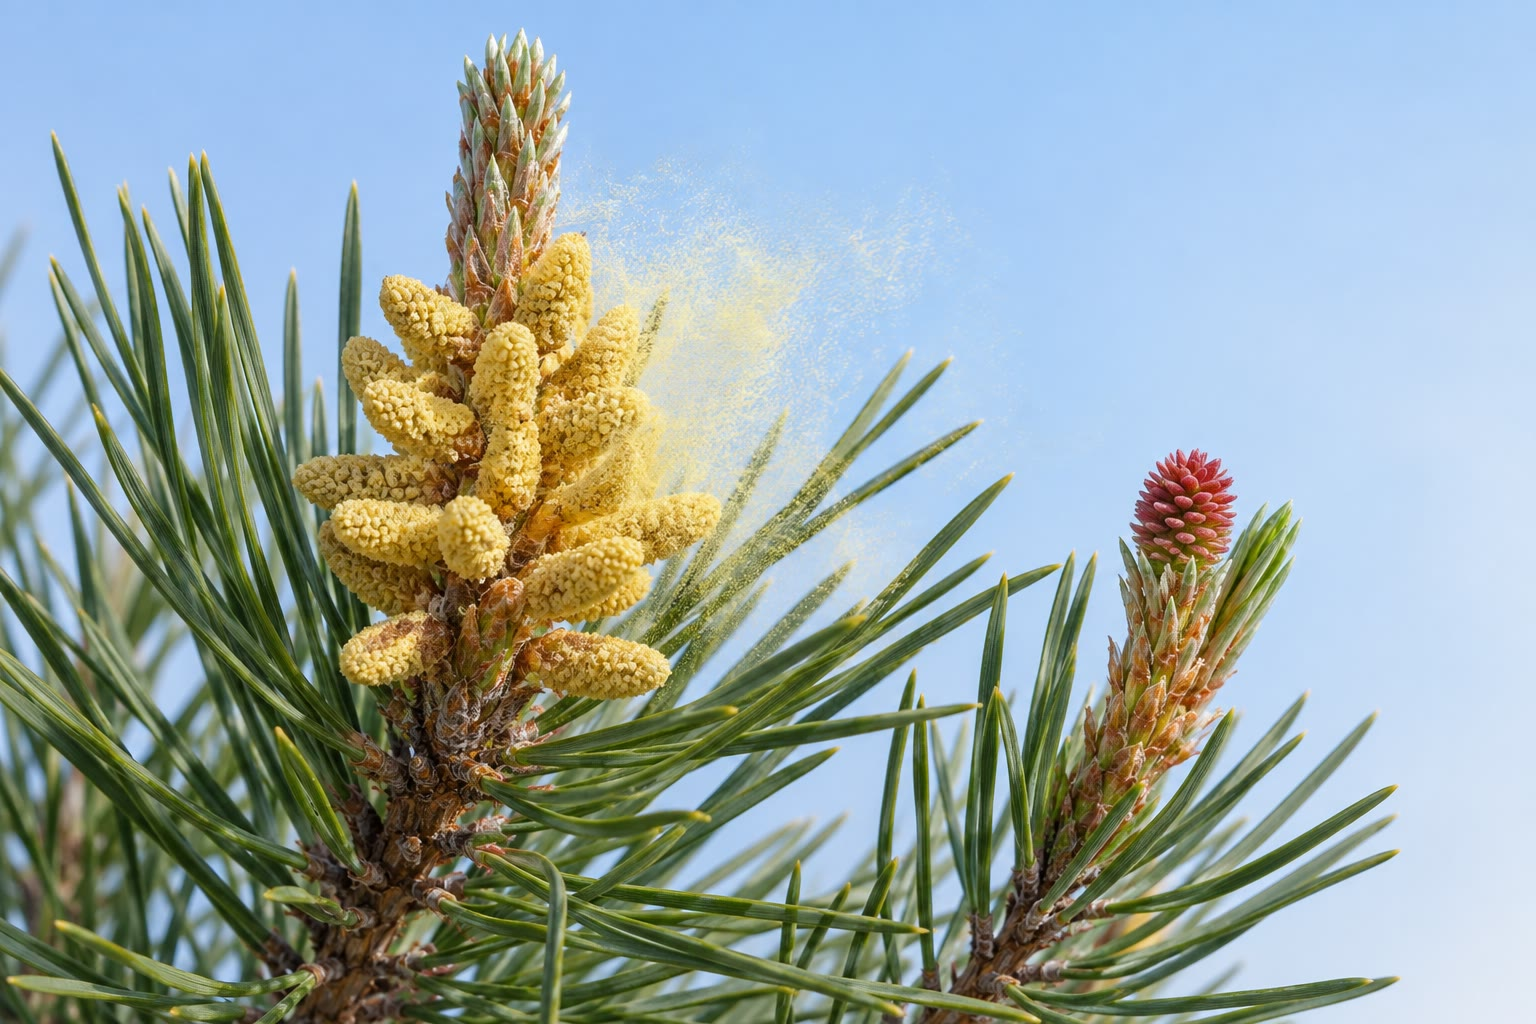
\includegraphics[width=0.6\linewidth]{images/book4/ai/b4-05-pine-cones.jpg}

{\small वसंत में चीड़ की एक शाखा: \omterm{def:b2:plant-life-cycles:heterospory}{पराग} झाड़ते पीले नर शंकुओं का एक
गुच्छ, और किसी दूसरी शाखा के सिरे पर एक छोटा लाल मादा शंकु, जिसके शल्क
उसे पकड़ने को खुले हैं।}
\end{omfigure}

\begin{example}[वायु में पराग]\label{ex:b2:plant-life-cycles:pollen}
चीड़ का कोई \omterm{def:b2:plant-life-cycles:heterospory}{पराग} कण, दो थैलियों सहित \qty{50}{\micro m} चौड़ा,
लगभग \qty{3}{cm/s} से गिरता है; कोई बड़ा वृक्ष एक ऋतु में कोई
$10^{11}$ कण छोड़ता है, जो तालाबों को पीला कर देने को पर्याप्त हैं। किसी
एक कण के किसी दिए हुए \omterm{def:b2:plant-life-cycles:heterospory}{बीजांड} पर उतरने की संभावना नन्ही है, और यह
रणनीति केवल संख्या के बल पर चलती है: वायु-परागण प्रति कण सस्ता है, पर
कणों में महँगा, और उन्हीं पौधों तक सीमित है जो अपनी ही जाति के झुंडों
में उगते हैं --- शंकुधारी, घास, बलूत। सपुष्पक
पौधों (\cref{ch:b2:angiosperm-reproduction}) ने \omterm{def:b2:plant-life-cycles:heterospory}{पराग} को प्राणियों से,
एक-एक कण सही पते पर, पहुँचाने का रास्ता ढूँढ़ लिया।
\end{example}

\section{स्थलीय पौधों में दिखती प्रवृत्तियाँ}

\begin{proposition}[चार प्रवृत्तियाँ]\label{prop:b2:plant-life-cycles:trends}
\index{युग्मकोद्भिद का ह्रास}
\omterm{def:b2:plant-life-cycles:moss}{मॉसों} से \omterm{def:b2:plant-life-cycles:fern}{फ़र्नों} तक और \omterm{def:b2:plant-life-cycles:fern}{फ़र्नों} से बीज-पौधों तक: (1) \omterm{def:b2:plant-life-cycles:cycles}{बीजाणुद्भिद} किसी
आश्रित डंठल से बढ़कर पूरा पौधा बन जाता है, और \omterm{def:b2:plant-life-cycles:cycles}{युग्मकोद्भिद} पौधे से
सिकुड़कर पपड़ी और फिर कुछ ही कोशिकाएँ रह जाता है; (2) समबीजाणुता
\omterm{def:b2:plant-life-cycles:heterospory}{विषमबीजाणुता} को जगह दे देती है, और मादा \omterm{def:b2:plant-life-cycles:cycles}{युग्मकोद्भिद} जनक पर ही रहता है;
(3) निषेचन सतही जल में तैरते शुक्राणुओं से हटकर किसी
\omterm{def:b2:plant-life-cycles:heterospory}{पराग} नलिका पर आ जाता है, इसलिए जनन को अब वर्षा नहीं चाहिए; (4)
प्रकीर्णन-इकाई बीजाणु से --- यानी दिन भर के भंडार वाली एक ही कोशिका से
--- हटकर बीज बन जाती है, यानी भोजन और आवरण सहित एक भ्रूण, जो प्रतीक्षा
कर सकता है। \omterm{def:b2:meiosis-heredity:meiosis}{द्विगुणित} पीढ़ी स्थल पर इसलिए पक्ष में रही कि कोई \omterm{def:b2:meiosis-heredity:meiosis}{द्विगुणित}
काया \omterm{def:b2:meiosis-heredity:vocabulary}{अप्रभावी} \omterm{def:b2:genome-diversification:mutation}{उत्परिवर्तनों} को ढँक लेती है, किसी संवहनी तंत्र के साथ
बड़ी और दीर्घजीवी हो सकती है, और इसलिए भी कि किसी ऊँचे \omterm{def:b2:plant-life-cycles:cycles}{बीजाणुद्भिद} पर
\omterm{def:b2:meiosis-heredity:meiosis}{अर्धसूत्री विभाजन} से बना बीजाणु किसी नीचे \omterm{def:b2:plant-life-cycles:cycles}{युग्मकोद्भिद} से तैरते युग्मक
से कहीं दूर जाता है। यह प्रवृत्ति सपुष्पक पौधों तक चलती है, जहाँ
मादा \omterm{def:b2:plant-life-cycles:cycles}{युग्मकोद्भिद} सात कोशिकाओं का है और बीज किसी फल में लिपटा है।
\end{proposition}

\begin{example}[समूहों की तुलना]\label{ex:b2:plant-life-cycles:table}
\begin{center}
\small
\begin{tabular}{p{2.3cm}p{3.1cm}p{3.1cm}p{3.3cm}}
\hline
 & \omterm{def:b2:plant-life-cycles:moss}{मॉस} & \omterm{def:b2:plant-life-cycles:fern}{फ़र्न} & शंकुधारी \\
\hline
प्रबल पीढ़ी & \omterm{def:b2:plant-life-cycles:cycles}{युग्मकोद्भिद} & \omterm{def:b2:plant-life-cycles:cycles}{बीजाणुद्भिद} & \omterm{def:b2:plant-life-cycles:cycles}{बीजाणुद्भिद} \\
\omterm{def:b2:plant-life-cycles:cycles}{युग्मकोद्भिद} & पत्तीदार प्ररोह, सेमी & \omterm{def:b2:plant-life-cycles:fern}{प्रोथैलस}, मिमी, स्वतंत्र & \omterm{def:b2:plant-life-cycles:heterospory}{पराग} कण (4 कोशिकाएँ); \omterm{def:b2:plant-life-cycles:heterospory}{बीजांड} की अंतर्वस्तु (हज़ारों कोशिकाएँ) \\
बीजाणु & एक प्रकार & एक प्रकार & \omterm{def:b2:plant-life-cycles:heterospory}{लघुबीजाणु}, \omterm{def:b2:plant-life-cycles:heterospory}{गुरुबीजाणु} \\
निषेचन & शुक्राणु जल में तैरते हैं & शुक्राणु जल में तैरते हैं & \omterm{def:b2:plant-life-cycles:heterospory}{पराग} नलिका \\
प्रकीर्णन-इकाई & बीजाणु & बीजाणु & बीज \\
संवहनी ऊतक & कोई नहीं & जाइलम, फ्लोएम & जाइलम, फ्लोएम, काष्ठ \\
\hline
\end{tabular}
\end{center}
\end{example}

\section{अभ्यास}

\begin{exercise}[$\star$]\label{exo:b2:plant-life-cycles:1}
\omterm{def:b2:plant-life-cycles:cycles}{युग्मकोद्भिद}, \omterm{def:b2:plant-life-cycles:cycles}{बीजाणुद्भिद}, बीजाणु और युग्मक की परिभाषा दीजिए, और बताइए
कि इन चारों में से हर एक किस प्रकार के विभाजन (समसूत्री या अर्धसूत्री) से बनता है।
\end{exercise}

\begin{exercise}[$\star$]\label{exo:b2:plant-life-cycles:2}
\omterm{def:b2:plant-life-cycles:fern}{फ़र्न} \emph{Ophioglossum reticulatum} की पर्ण-कोशिकाओं में \num{1260}
गुणसूत्र हैं। किसी बीजाणु में, किसी \omterm{def:b2:plant-life-cycles:fern}{प्रोथैलस}
कोशिका में, किसी शुक्राणु में, किसी अंडाणु में, किसी युग्मनज में कितने?
\end{exercise}

\begin{exercise}[$\star$]\label{exo:b2:plant-life-cycles:3}
\omterm{def:b2:plant-life-cycles:moss}{मॉस} का हरा गद्दा कौन-सी पीढ़ी है? संपुट वाला भूरा डंठल?
कोई \omterm{def:b2:plant-life-cycles:fern}{फ़र्न} पत्रक? कोई \omterm{def:b2:plant-life-cycles:fern}{प्रोथैलस}? कोई \omterm{def:b2:plant-life-cycles:heterospory}{पराग} कण? किसी चीड़-बीज
का भोजन-भंडार? किसी चीड़-बीज का भ्रूण?
\end{exercise}

\begin{exercise}[$\star$]\label{exo:b2:plant-life-cycles:4}
\omterm{def:b2:plant-life-cycles:cycles}{जीवन-चक्र} के तीनों प्रकार बताइए और हर एक के लिए एक जीव दीजिए।
हर एक में \omterm{def:b2:meiosis-heredity:meiosis}{अर्धसूत्री विभाजन} कहाँ होता है?
\end{exercise}

\begin{exercise}[$\star\star$]\label{exo:b2:plant-life-cycles:5}
\omterm{def:b2:plant-life-cycles:moss}{मॉस} का शुक्राणु \qty{100}{\micro m/s} से तैरता है। \qty{3}{cm} दूर की
किसी \omterm{def:b2:plant-life-cycles:moss}{स्त्रीधानी} तक पहुँचने में उसे कितना समय लगता है? कोई ओस-झिल्ली
सूर्योदय के \qty{20}{min} बाद वाष्पित हो जाती है: निषेचन की अधिकतम परास
क्या है? \omterm{def:b2:plant-life-cycles:moss}{मॉस} निवहों के आकार पर टिप्पणी कीजिए।
\end{exercise}

\begin{exercise}[$\star\star$]\label{exo:b2:plant-life-cycles:6}
\qty{15}{\micro m} त्रिज्या और \qty{1100}{kg/m^3} घनत्व के किसी
\omterm{def:b2:plant-life-cycles:fern}{फ़र्न} बीजाणु की वायु में अवसादन-चाल निकालिए ($\eta =
\qty{1.8e-5}{Pa.s}$, $\rho_{\text{वायु}} = \qty{1.2}{kg/m^3}$), और
\qty{0.5}{m} से \qty{2}{m/s} की वायु में उसकी तय की दूरी।
\qty{5}{mg} द्रव्यमान के किसी चीड़-बीज के लिए, जिसका पंख उसे
\qty{0.8}{m/s} की उतरने की चाल देता है और जो \qty{20}{m} से झड़ता है, यह दोहराइए।
\end{exercise}

\begin{exercise}[$\star\star$]\label{exo:b2:plant-life-cycles:7}
किसी \omterm{def:b2:plant-life-cycles:fern}{फ़र्न} पत्रक पर \num{40} बीजाणुधानियों के \num{200} \omterm{def:b2:plant-life-cycles:fern}{सोरस} हैं, और हर
\omterm{def:b2:plant-life-cycles:fern}{बीजाणुधानी} \num{64} बीजाणु बनाती है। प्रति पत्रक कितने बीजाणु? यदि
$10^{5}$ में एक बीजाणु \omterm{def:b2:plant-life-cycles:fern}{प्रोथैलस} बने और \num{50} में एक \omterm{def:b2:plant-life-cycles:fern}{प्रोथैलस}
कोई \omterm{def:b2:plant-life-cycles:cycles}{बीजाणुद्भिद} दे, तो एक पत्रक से कितने नए \omterm{def:b2:plant-life-cycles:fern}{फ़र्न}
निकलते हैं?
\end{exercise}

\begin{exercise}[$\star\star$]\label{exo:b2:plant-life-cycles:8}
समझाइए कि \omterm{def:b2:plant-life-cycles:heterospory}{विषमबीजाणुता} बीज की पूर्वशर्त क्यों है, और कोई
समबीजाणुक पौधा अपने मादा \omterm{def:b2:plant-life-cycles:cycles}{युग्मकोद्भिद} को किसी
\omterm{def:b2:plant-life-cycles:heterospory}{बीजांड} में क्यों नहीं घेर सकता।
\end{exercise}

\begin{exercise}[$\star\star$]\label{exo:b2:plant-life-cycles:9}
किसी \omterm{def:b2:plant-life-cycles:fern}{फ़र्न} बीजाणु (\qty{15}{\micro m} त्रिज्या का गोला, घनत्व
\qty{1100}{kg/m^3}) और किसी चीड़-बीज (\qty{5}{mg}) की प्रकीर्णन-इकाइयों
के रूप में तुलना कीजिए: द्रव्यमान, ऊर्जा-अंश (शुष्क पदार्थ
\qty{20}{kJ/g}, \qty{50}{\%} शुष्क लीजिए), और उतरने पर हर एक क्या कर
सकता है और क्या नहीं।
\end{exercise}

\begin{exercise}[$\star\star\star$]\label{exo:b2:plant-life-cycles:10}
कोई चीड़ किसी वन पर $10^{11}$ \omterm{def:b2:plant-life-cycles:heterospory}{पराग} कण छोड़ता है; \omterm{def:b2:plant-life-cycles:heterospory}{बीजांड}
की ऊँचाई पर वे कण \qty{1}{km^2} पर \qty{20}{m} गहरी परत में फैले हैं।
\omterm{def:b2:plant-life-cycles:heterospory}{पराग} की सांद्रता (कण प्रति घन
मीटर), \qty{2}{m/s} की वायु में किसी \omterm{def:b2:plant-life-cycles:heterospory}{बीजांड} के
बीजांडद्वारी छिद्र (\qty{0.1}{mm^2}) से प्रति सेकंड गुज़रते कणों की
संख्या, और किसी \omterm{def:b2:plant-life-cycles:heterospory}{बीजांड} को एक कण मिलने का काल आँकिए। यह शंकु खुलने के
समय के बारे में क्या कहता है?
\end{exercise}

\begin{exercise}[$\star\star\star$]\label{exo:b2:plant-life-cycles:11}
तीन कारण बताइए कि \omterm{def:b2:meiosis-heredity:meiosis}{द्विगुणित} पीढ़ी स्थलीय पौधों के \omterm{def:b2:plant-life-cycles:cycles}{जीवन-चक्र} पर
क्यों छा गई, और एक कारण कि \omterm{def:b2:meiosis-heredity:meiosis}{अगुणित} पीढ़ी
पूरी तरह लुप्त क्यों नहीं हुई।
\end{exercise}

\begin{exercise}[$\star\star\star$]\label{exo:b2:plant-life-cycles:12}
हॉफ़माइस्टर ने गुणसूत्रों के ज्ञात होने से पहले काम किया था। समझाइए कि
वे केवल सूक्ष्मदर्शन और संवर्धन से \omterm{def:b2:plant-life-cycles:cycles}{पीढ़ी-एकांतरण} के बारे में
क्या स्थापित कर सके और क्या नहीं, और गुणसूत्र-गणनाओं ने उसमें क्या
जोड़ा।
\end{exercise}

\section{समस्या: बीजाणु से बीज तक}

\begin{problem}[{सप्तांत समस्या --- किसी फ़र्न और किसी चीड़ के जननीय
अंकगणित की तुलना, बीजाणुओं तथा पराग कणों की संख्या से लेकर उनके
प्रकीर्णन, युग्मकोद्भिदों की नियति और किसी बीज की क़ीमत तक, और अंत उन
प्रवर्ध्यों की संख्या पर जो हर पौधे को एक प्रतिस्थापन के लिए बनाने
पड़ते हैं}]
\label{pb:b2:plant-life-cycles:1}
किसी \omterm{def:b2:plant-life-cycles:fern}{फ़र्न} पौधे पर \num{10} उर्वर पत्रक हैं, और हर एक पर \num{40}
बीजाणुधानियों के \num{200} \omterm{def:b2:plant-life-cycles:fern}{सोरस} हैं, जिनमें से हर एक \num{64} बीजाणु
बनाती है। बीजाणु: त्रिज्या \qty{15}{\micro m}, घनत्व \qty{1100}{kg/m^3}।
कोई चीड़ अपने जीवन भर में $2\times 10^{4}$ मादा शंकुओं जितने \omterm{def:b2:plant-life-cycles:heterospory}{बीजांड}
बनाता है --- प्रति शंकु \num{100} \omterm{def:b2:plant-life-cycles:heterospory}{बीजांड} लीजिए --- और प्रति वर्ष
$10^{11}$ \omterm{def:b2:plant-life-cycles:heterospory}{पराग} कण। बीज: \qty{5}{mg}, \qty{50}{\%} शुष्क पदार्थ
\qty{20}{kJ/g} पर। वायु: $\eta = \qty{1.8e-5}{Pa.s}$, $\rho =
\qty{1.2}{kg/m^3}$; $g = \qty{9.81}{m/s^2}$।

\medskip
\noindent\textbf{भाग I --- \omterm{def:b2:plant-life-cycles:fern}{फ़र्न} के बीजाणु।}
\begin{enumerate}
  \item वह पौधा एक ऋतु में कितने बीजाणु झाड़ता है, निकालिए।
  \item एक बीजाणु का और पूरी फ़सल का द्रव्यमान निकालिए।
  \item उस बीजाणु की वायु में अवसादन-चाल निकालिए।
  \item \qty{0.5}{m} पर के पत्रकों से \qty{1.5}{m/s} की वायु में वे
        बीजाणु कितनी दूर जाते हैं? वे कितने बड़े क्षेत्र (उसी त्रिज्या
        की चक्रिका) पर फैलते हैं, और प्रति वर्ग मीटर कितने उतरते हैं?
  \item समझाइए कि विक्षोभ कुछ बीजाणुओं को कहीं दूर क्यों ले जाता है,
        और इसका किसी नए द्वीप के बसने के लिए क्या अर्थ है।
  \item एक बीजाणु का (\qty{50}{\%} शुष्क पदार्थ \qty{20}{kJ/g} पर) और
        पूरी फ़सल का ऊर्जा-अंश निकालिए, और उसकी तुलना
        एक चीड़-बीज की ऊर्जा से कीजिए।
\end{enumerate}

\medskip
\noindent\textbf{भाग II --- \omterm{def:b2:plant-life-cycles:cycles}{युग्मकोद्भिद}।}
$2\times 10^{4}$ में एक बीजाणु इतनी नम मिट्टी पर उतरता है कि वह
\omterm{def:b2:plant-life-cycles:fern}{प्रोथैलस} बन सके; कोई \omterm{def:b2:plant-life-cycles:fern}{प्रोथैलस} \num{6} सप्ताह जीता है और उसे निषेचन के
लिए एक गीली रात चाहिए --- प्रति सप्ताह प्रायिकता $0.2$; कोई
निषेचित \omterm{def:b2:plant-life-cycles:fern}{प्रोथैलस} $0.5$ प्रायिकता से एक नया \omterm{def:b2:plant-life-cycles:cycles}{बीजाणुद्भिद}
देता है; और कोई नया \omterm{def:b2:plant-life-cycles:cycles}{बीजाणुद्भिद} $0.02$ प्रायिकता से
वयस्कता तक बचता है।
\begin{enumerate}[resume]
  \item उस पौधे की फ़सल कितने \omterm{def:b2:plant-life-cycles:fern}{प्रोथैलस} बनाती है?
  \item किसी \omterm{def:b2:plant-life-cycles:fern}{प्रोथैलस} को अपने छह सप्ताहों में कम से कम एक गीली रात
        मिलने की प्रायिकता निकालिए।
  \item एक ऋतु की फ़सल से बनने वाले वयस्क \omterm{def:b2:plant-life-cycles:fern}{फ़र्नों} की
        प्रत्याशित संख्या निकालिए।
  \item यदि जनक \num{30} वर्ष जीए, तो वह कितनी वयस्क संतति छोड़ता है,
        और यह \omterm{def:b2:plant-life-cycles:fern}{फ़र्न} की आबादी के बारे में क्या
        कहता है?
  \item \omterm{def:b2:plant-life-cycles:fern}{फ़र्न} का शुक्राणु \qty{100}{\micro m/s} से तैरता है और किसी \omterm{def:b2:plant-life-cycles:fern}{प्रोथैलस}
        की स्त्रीधानियाँ उसकी अपनी पुंधानियों से \qty{1}{mm} दूर हैं।
        स्व-निषेचन में कितना समय लगता है? फिर भी अनेक \omterm{def:b2:plant-life-cycles:fern}{फ़र्न} उससे
        क्यों बचते हैं (एक क्रियाविधि दीजिए)?
  \item \omterm{def:b2:plant-life-cycles:fern}{प्रोथैलस} किस अर्थ में फ़र्न-चक्र की सबसे कमज़ोर
        कड़ी है?
\end{enumerate}

\medskip
\noindent\textbf{भाग III --- चीड़ का \omterm{def:b2:plant-life-cycles:heterospory}{पराग}।}
\begin{enumerate}[resume]
  \item कोई \omterm{def:b2:plant-life-cycles:heterospory}{पराग} कण \qty{25}{\micro m} त्रिज्या का ऐसा गोला है जिसका
        \omterm{def:b2:meiosis-heredity:vocabulary}{प्रभावी} घनत्व \qty{600}{kg/m^3} है (वायु-थैलियाँ मिलाकर)।
        उसकी अवसादन-चाल निकालिए।
  \item \qty{15}{m} पर के किसी शंकु से \qty{3}{m/s} की वायु में वह
        कितनी दूर जाता है?
  \item वे $10^{11}$ कण \qty{1}{km^2} वन में \qty{20}{m} की गहराई तक
        फैले हैं। सांद्रता निकालिए।
  \item कोई बीजांडद्वार \qty{2}{m/s} की वायु के सामने
        \qty{0.1}{mm^2} का छिद्र प्रस्तुत करता है। उसमें प्रति घंटा
        प्रवेश करते कणों की संख्या और पहला कण मिलने का काल निकालिए।
  \item समझाइए कि वन से \qty{5}{km} दूर का कोई अकेला चीड़ लगभग कोई बीज
        क्यों नहीं बनाता, और वायु-परागित जातियाँ झुंडों में क्यों
        उगती हैं।
  \item संख्याओं की तुलना कीजिए: यदि उस वन में \num{1000} चीड़ हों और
        हर एक पर \num{2000} \omterm{def:b2:plant-life-cycles:heterospory}{बीजांड}, तो वह प्रति \omterm{def:b2:plant-life-cycles:heterospory}{बीजांड} कितने \omterm{def:b2:plant-life-cycles:heterospory}{पराग} कण
        बनाता है?
\end{enumerate}

\medskip
\noindent\textbf{भाग IV --- चीड़ के बीज।}
उस वृक्ष के \omterm{def:b2:plant-life-cycles:heterospory}{बीजांडों} में से \qty{60}{\%} परागित होते हैं और उनमें से
\qty{80}{\%} कोई बीज भर देते हैं; कोई बीज $0.05$ प्रायिकता से अंकुर बनता
है और कोई अंकुर $0.01$ प्रायिकता से वयस्क।
\begin{enumerate}[resume]
  \item वह वृक्ष अपने जीवन में कितने बीज बनाता है, और उनका कुल
        द्रव्यमान तथा ऊर्जा, निकालिए।
  \item कोई पंखदार बीज \qty{0.8}{m/s} से उतरता है। \qty{20}{m} से
        \qty{3}{m/s} की वायु में वह कितनी दूर जाता है? \omterm{def:b2:plant-life-cycles:heterospory}{पराग} से
        तुलना कीजिए।
  \item वयस्क संतति की प्रत्याशित संख्या निकालिए और
        \omterm{def:b2:plant-life-cycles:fern}{फ़र्न} की संख्या से तुलना कीजिए।
  \item वह वृक्ष प्रति वयस्क संतान कितनी ऊर्जा लगाता है, और
        \omterm{def:b2:plant-life-cycles:fern}{फ़र्न} प्रति वयस्क संतान कितनी (केवल बीजाणु), निकालिए और तुलना कीजिए।
  \item \omterm{def:b2:plant-life-cycles:fern}{फ़र्न} का बीजाणु कुछ सप्ताह प्रतीक्षा कर सकता है; चीड़ का बीज कई
        वर्ष। ऊर्जा के आँकड़ों से समझाइए कि बीज प्रसुप्ति क्यों झेल
        सकता है और बीजाणु क्यों नहीं।
  \item दो लाभ बताइए जो बीज को उसकी क़ीमत के योग्य बनाते हैं, और दो
        परिस्थितियाँ जिनमें \omterm{def:b2:plant-life-cycles:fern}{फ़र्न} की रणनीति बेहतर है।
  \item परिणाम बताइए: \omterm{def:b2:plant-life-cycles:fern}{फ़र्न} के लिए और चीड़ के लिए प्रति वयस्क संतान
        प्रवर्ध्यों की संख्या, और हर एक प्रति वयस्क संतान कितनी ऊर्जा
        ख़र्च करता है।
\end{enumerate}
\end{problem}
